\documentclass[11pt,a4paper]{article}
\usepackage[utf8]{inputenc}
\usepackage[T1]{fontenc}
\usepackage[margin=2.4cm]{geometry}
\usepackage{graphicx}
\usepackage{booktabs}
\usepackage{array}
\usepackage{longtable}
\usepackage{float}
\usepackage{subcaption}
\usepackage{hyperref}
\usepackage{amsmath}
\usepackage{caption}
\usepackage{siunitx}
\graphicspath{{../../data/plots/}}

\title{A121 Sleep Radar Lens Experiments\\\large Overnight comparison of plano-convex, FZP, and flat-cover configurations with Garmin reference data}
\author{}
\date{June 2026}

\begin{document}
\maketitle

\begin{abstract}
This report summarizes three overnight A121 radar sleep recordings and two short follow-up bench tests performed while changing the front-end optical/mechanical configuration: a plano-convex lens (night 1\_1), a Fresnel zone plate (FZP) lens (night 2), and a flat cover that behaved approximately like a no-lens condition (night 3). Garmin heart-rate (HR), respiration-rate (RR), and sleep-stage overlays were used as the main external reference. A key result of the analysis is that raw radar \texttt{peak\_amplitude} cannot be interpreted as chest-signal strength in this setup, because the radar was placed near the bed edge and the dominant reflector was often closer than the tracked subject distance. The most meaningful comparison therefore comes from Garmin agreement and from the plausibility/stability of the radar-derived sleep metrics. Night 3, despite having no focusing lens, produced the closest HR agreement to Garmin, while nights 1\_1 and 2 showed larger HR bias and heuristic REM$\rightarrow$deep transitions not present in Garmin. The short \SI{2}{m} retest showed only a small amplitude increase with the plano-convex lens compared with no lens, but the lens produced more plausible HR estimates.
\end{abstract}

\section{Background and framing}
Acconeer's lens design documentation notes that dielectric lenses are mainly used to shape the radiation pattern, increase gain, narrow the beamwidth, and in some cases suppress unwanted reflections. The same documentation presents both a plano-convex example lens and an FZP example lens for A121-class hardware, and explicitly notes that focal distance may require tuning because the optimum can shift due to the radome, housing, material tolerances, and nearby mechanics. This point is directly relevant here because the experiments were performed in a bedroom geometry with the radar mounted near the bed edge rather than in a controlled free-space test fixture.

\paragraph{Interpretation rule used throughout this report.}
\begin{quote}
\textbf{Raw \texttt{peak\_amplitude} is treated only as a dominant-return engineering metric, not as a direct proxy for chest reflection strength or physiological signal quality.} The reason is that the strongest radar return could originate from the bed edge, mattress, bedding, or another static reflector rather than the subject.
\end{quote}

This framing is important because the raw peak amplitudes differed by more than an order of magnitude between nights, yet the strongest returns were often not spatially aligned with the tracked target distance.

\section{Experimental conditions}
Table~\ref{tab:nights} summarizes the three overnight recordings used in the comparison. Night 3 was interrupted, so it contains only about three hours of usable data. The Garmin overlay plots and the radar sleep-score JSON sidecars were generated for all three nights.

\begin{table}[H]
\centering
\caption{Overnight recordings and hardware condition.}
\label{tab:nights}
\begin{tabular}{@{}lllll@{}}
\toprule
Night & Date & Front-end condition & Recording length & Note \\
\midrule
1\_1 & 2026-06-08 & Plano-convex lens & 6.95 h & Full night \\
2 & 2026-06-09 & FZP lens & 6.48 h & Full night \\
3 & 2026-06-10 & Flat cover / effectively no lens & 3.56 h & Interrupted recording \\
\bottomrule
\end{tabular}
\end{table}

The A121 lens documentation is useful for interpreting these tests:
\begin{itemize}
    \item dielectric lenses can increase gain and narrow the beam,
    \item the plano-convex and FZP lenses are both valid A121-compatible example designs,
    \item FZP lenses are mechanically thinner and their thickness is less coupled to diameter,
    \item the effective focal point can shift because of radome/housing effects and nearby mechanics.
\end{itemize}
These points make aiming and lens-to-radar spacing critical, especially in a bed-edge mounting geometry.

\section{Analysis method}
The overnight data were processed with the repository's A121 sleep-analysis pipeline. For each night the following outputs were generated and used here:
\begin{itemize}
    \item gated radar HR/RR trends,
    \item radar sleep-phase heuristic and radar sleep score,
    \item Garmin HR/RR overlays,
    \item radar sleep-parameter JSON sidecars,
    \item diagnostic comparison plots.
\end{itemize}

The following metrics were extracted:
\begin{enumerate}
    \item radar sleep score, total sleep time, efficiency, and estimated resting HR,
    \item mean and median HR/RR compared against Garmin,
    \item sleep-stage duration sums (where available from the analysis session),
    \item direct REM$\rightarrow$deep transition counts,
    \item dominant-return peak amplitude and its spatial alignment to the tracked target distance,
    \item short timed lens vs. no-lens retest diagnostics at roughly \SI{2}{m}.
\end{enumerate}

Estimated resting HR was added to the automatic radar sleep JSON files and defined as the \emph{10th percentile of quiet, non-awake radar HR windows inside the inferred sleep interval}. This makes it more robust than taking a raw minimum while still approximating the lower resting envelope overnight.

\section{Primary overnight results}

\subsection{Radar-only sleep summary}
Table~\ref{tab:radarsleep} summarizes the radar-inferred overnight sleep metrics.

\begin{table}[H]
\centering
\caption{Radar sleep summary from the generated JSON sidecars.}
\label{tab:radarsleep}
\resizebox{\textwidth}{!}{%
\begin{tabular}{@{}lrrrrr@{}}
\toprule
Night & Score & Total sleep [min] & Efficiency [\%] & Estimated resting HR [bpm] & Quality \\
\midrule
1\_1 & 74 & 364.5 & 93.8 & 52.7 & Fair \\
2 & 71 & 342.5 & 95.0 & 51.9 & Fair \\
3 & 49 & 154.0 & 85.8 & 50.8 & Poor \\
\bottomrule
\end{tabular}%
}
\end{table}

Night 3 scored substantially worse mainly because the recording was interrupted and therefore short; the score was capped by duration. The estimated resting HR remained internally consistent across nights, staying in the low-50 bpm range.

\subsection{Heart-rate comparison against Garmin}
Garmin agreement is the most important outcome because it is much less sensitive to the bed-edge reflector issue than raw radar amplitude. Table~\ref{tab:hr} uses the sleep-only comparison windows discussed during the analysis session.

\begin{table}[H]
\centering
\caption{Sleep-only heart-rate comparison between radar and Garmin.}
\label{tab:hr}
\resizebox{\textwidth}{!}{%
\begin{tabular}{@{}lrrrrrr@{}}
\toprule
Night & Radar mean & Radar median & Garmin mean & Garmin median & Mean bias & Median bias \\
 & [bpm] & [bpm] & [bpm] & [bpm] & radar$-$Garmin & radar$-$Garmin \\
\midrule
1\_1 & 55.5 & 55.2 & 57.4 & 57.0 & -1.9 & -1.8 \\
2 & 55.1 & 54.6 & 58.3 & 57.0 & -3.3 & -2.4 \\
3 & 53.8 & 53.3 & 53.6 & 52.0 & +0.1 & +1.3 \\
\bottomrule
\end{tabular}%
}
\end{table}

The HR comparison shows the clearest practical result of the experiment: the flat-cover night (night 3) matched Garmin best, while the two lensed nights under-read HR on average. This does \emph{not} prove that the flat cover is universally better than a lens; it does show that the tested lens geometries did not automatically translate into better overnight physiological agreement in this mounting arrangement.

\subsection{Respiration-rate comparison against Garmin}
RR agreement was generally closer than HR agreement. Table~\ref{tab:rr} summarizes the values used during the analysis.

\begin{table}[H]
\centering
\caption{Sleep-only respiration-rate comparison between radar and Garmin.}
\label{tab:rr}
\resizebox{\textwidth}{!}{%
\begin{tabular}{@{}lrrrrrr@{}}
\toprule
Night & Radar mean & Radar median & Garmin mean & Garmin median & Mean bias & Median bias \\
 & [brpm] & [brpm] & [brpm] & [brpm] & radar$-$Garmin & radar$-$Garmin \\
\midrule
1\_1 & 13.6 & 14.2 & 14.0 & 14.4 & -0.4 & -0.2 \\
2 & 14.6 & 14.9 & 14.2 & 14.4 & +0.4 & +0.5 \\
3 & 14.3 & 14.3 & 14.0 & 14.1 & +0.3 & +0.2 \\
\bottomrule
\end{tabular}%
}
\end{table}

RR stayed within about half a breath per minute of Garmin on average for all three nights. This is a stronger and more stable result than the raw peak-amplitude comparison.

\subsection{Sleep-stage duration comparison}
For nights 1\_1 and 2, the analysis session retained quantitative radar-vs-Garmin sleep-stage duration sums extracted from the Garmin FIT stage data. These values are shown in Table~\ref{tab:stages}. Night 3 was interrupted and is therefore discussed primarily through the overlay plot and radar-only sleep summary.

\begin{table}[H]
\centering
\caption{Sleep-stage duration sums for nights 1\_1 and 2. Positive difference means radar assigned more time to that stage than Garmin.}
\label{tab:stages}
\resizebox{\textwidth}{!}{%
\begin{tabular}{@{}llrrrr@{}}
\toprule
Night & Source & Awake [min] & Light [min] & Deep [min] & REM [min] \\
\midrule
1\_1 & Radar & 24.0 & 212.5 & 78.5 & 73.5 \\
1\_1 & Garmin & 40.0 & 222.0 & 57.0 & 47.0 \\
1\_1 & Difference & -16.0 & -9.5 & +21.5 & +26.5 \\
\midrule
2 & Radar & 18.0 & 191.0 & 58.0 & 93.5 \\
2 & Garmin & 5.0 & 211.0 & 18.0 & 117.0 \\
2 & Difference & +13.0 & -20.0 & +40.0 & -23.5 \\
\bottomrule
\end{tabular}%
}
\end{table}

Two additional stage-related observations were important:
\begin{itemize}
    \item Nights 1\_1 and 2 contained direct radar REM$\rightarrow$deep transitions (two such transitions on each night), while Garmin showed zero direct REM$\rightarrow$deep transitions in those same nights.
    \item This suggests that at least part of the radar stage disagreement came from the heuristic classifier rather than from the raw HR/RR tracking alone.
\end{itemize}

\section{Why peak amplitude must be interpreted carefully}
The raw peak-amplitude plot across nights is striking: the median dominant return rises from roughly \num{1.7e3} in night 1\_1 to \num{1.75e4} in night 2 and \num{2.36e4} in night 3. However, Table~\ref{tab:peak} shows why this cannot be interpreted as ``better chest signal''.

\begin{table}[H]
\centering
\caption{Dominant-return amplitude and target-alignment diagnostics from the gated sleep-vitals CSV files.}
\label{tab:peak}
\resizebox{\textwidth}{!}{%
\begin{tabular}{@{}lrrrrrr@{}}
\toprule
Night & Peak amp median & Peak amp mean & Median target dist & Median peak dist & Median $|\Delta d|$ & Fraction with $|\Delta d|\leq$0.10 m \\
 & [a.u.] & [a.u.] & [m] & [m] & [m] & [-] \\
\midrule
1\_1 & 1665.2 & 3079.7 & 0.37 & 0.15 & 0.16 & 0.316 \\
2 & 17515.5 & 17659.7 & 0.44 & 0.12 & 0.32 & 0.012 \\
3 & 23574.3 & 23240.3 & 0.22 & 0.10 & 0.12 & 0.384 \\
\bottomrule
\end{tabular}%
}
\end{table}

The median dominant-return distance was much closer than the tracked target distance on all nights, especially on night 2. The FZP night is the clearest example: despite a median peak amplitude above \num{1.7e4}, only about \SI{1.2}{\percent} of windows had the dominant peak within \SI{10}{cm} of the target. This makes it highly likely that the large peak came from the bed edge or another nearby reflector rather than from the subject.

This is the reason for the specific presentation used in this report:
\begin{enumerate}
    \item Garmin HR/RR agreement is treated as the \textbf{primary outcome},
    \item sleep-stage agreement is treated as the \textbf{secondary outcome},
    \item raw peak amplitude is treated only as a \textbf{contextual engineering variable}. 
\end{enumerate}

\section{Short follow-up retest at approximately \SI{2}{m}}
A short retest was performed after the overnight analysis to check whether the plano-convex lens behaved more sensibly at a longer distance, where aiming is easier. One \SI{90}{s} sample was recorded with the lens and one without the lens.

\begin{table}[H]
\centering
\caption{Short \SI{2}{m} timed retest: lens vs. no lens.}
\label{tab:2mtest}
\resizebox{\textwidth}{!}{%
\begin{tabular}{@{}lrrrrrr@{}}
\toprule
Condition & Target dist [m] & Avg peak amp & Batch HR & Batch HR conf. & Weighted HR & Weighted HR conf. \\
\midrule
Plano-convex lens & 1.862 & 556 & 62.5 & 12.5 & 54.5 & 8.6 \\
No lens & 1.682 & 491 & 102.1 & 6.7 & 83.2 & 5.8 \\
\bottomrule
\end{tabular}%
}
\end{table}

The lens increased average peak amplitude only modestly (about \SI{13}{\percent}), so this was not a dramatic gain result. However, the lens case produced a much more plausible HR estimate than the no-lens case. This again supports the main argument of the report: \emph{amplitude alone is not the right decision metric}. A configuration can have only a small amplitude advantage yet still produce more believable physiology.

\section{Plots}
The generated plots are included below because the time-domain behavior is at least as informative as the summary tables.

\begin{figure}[p]
    \centering
    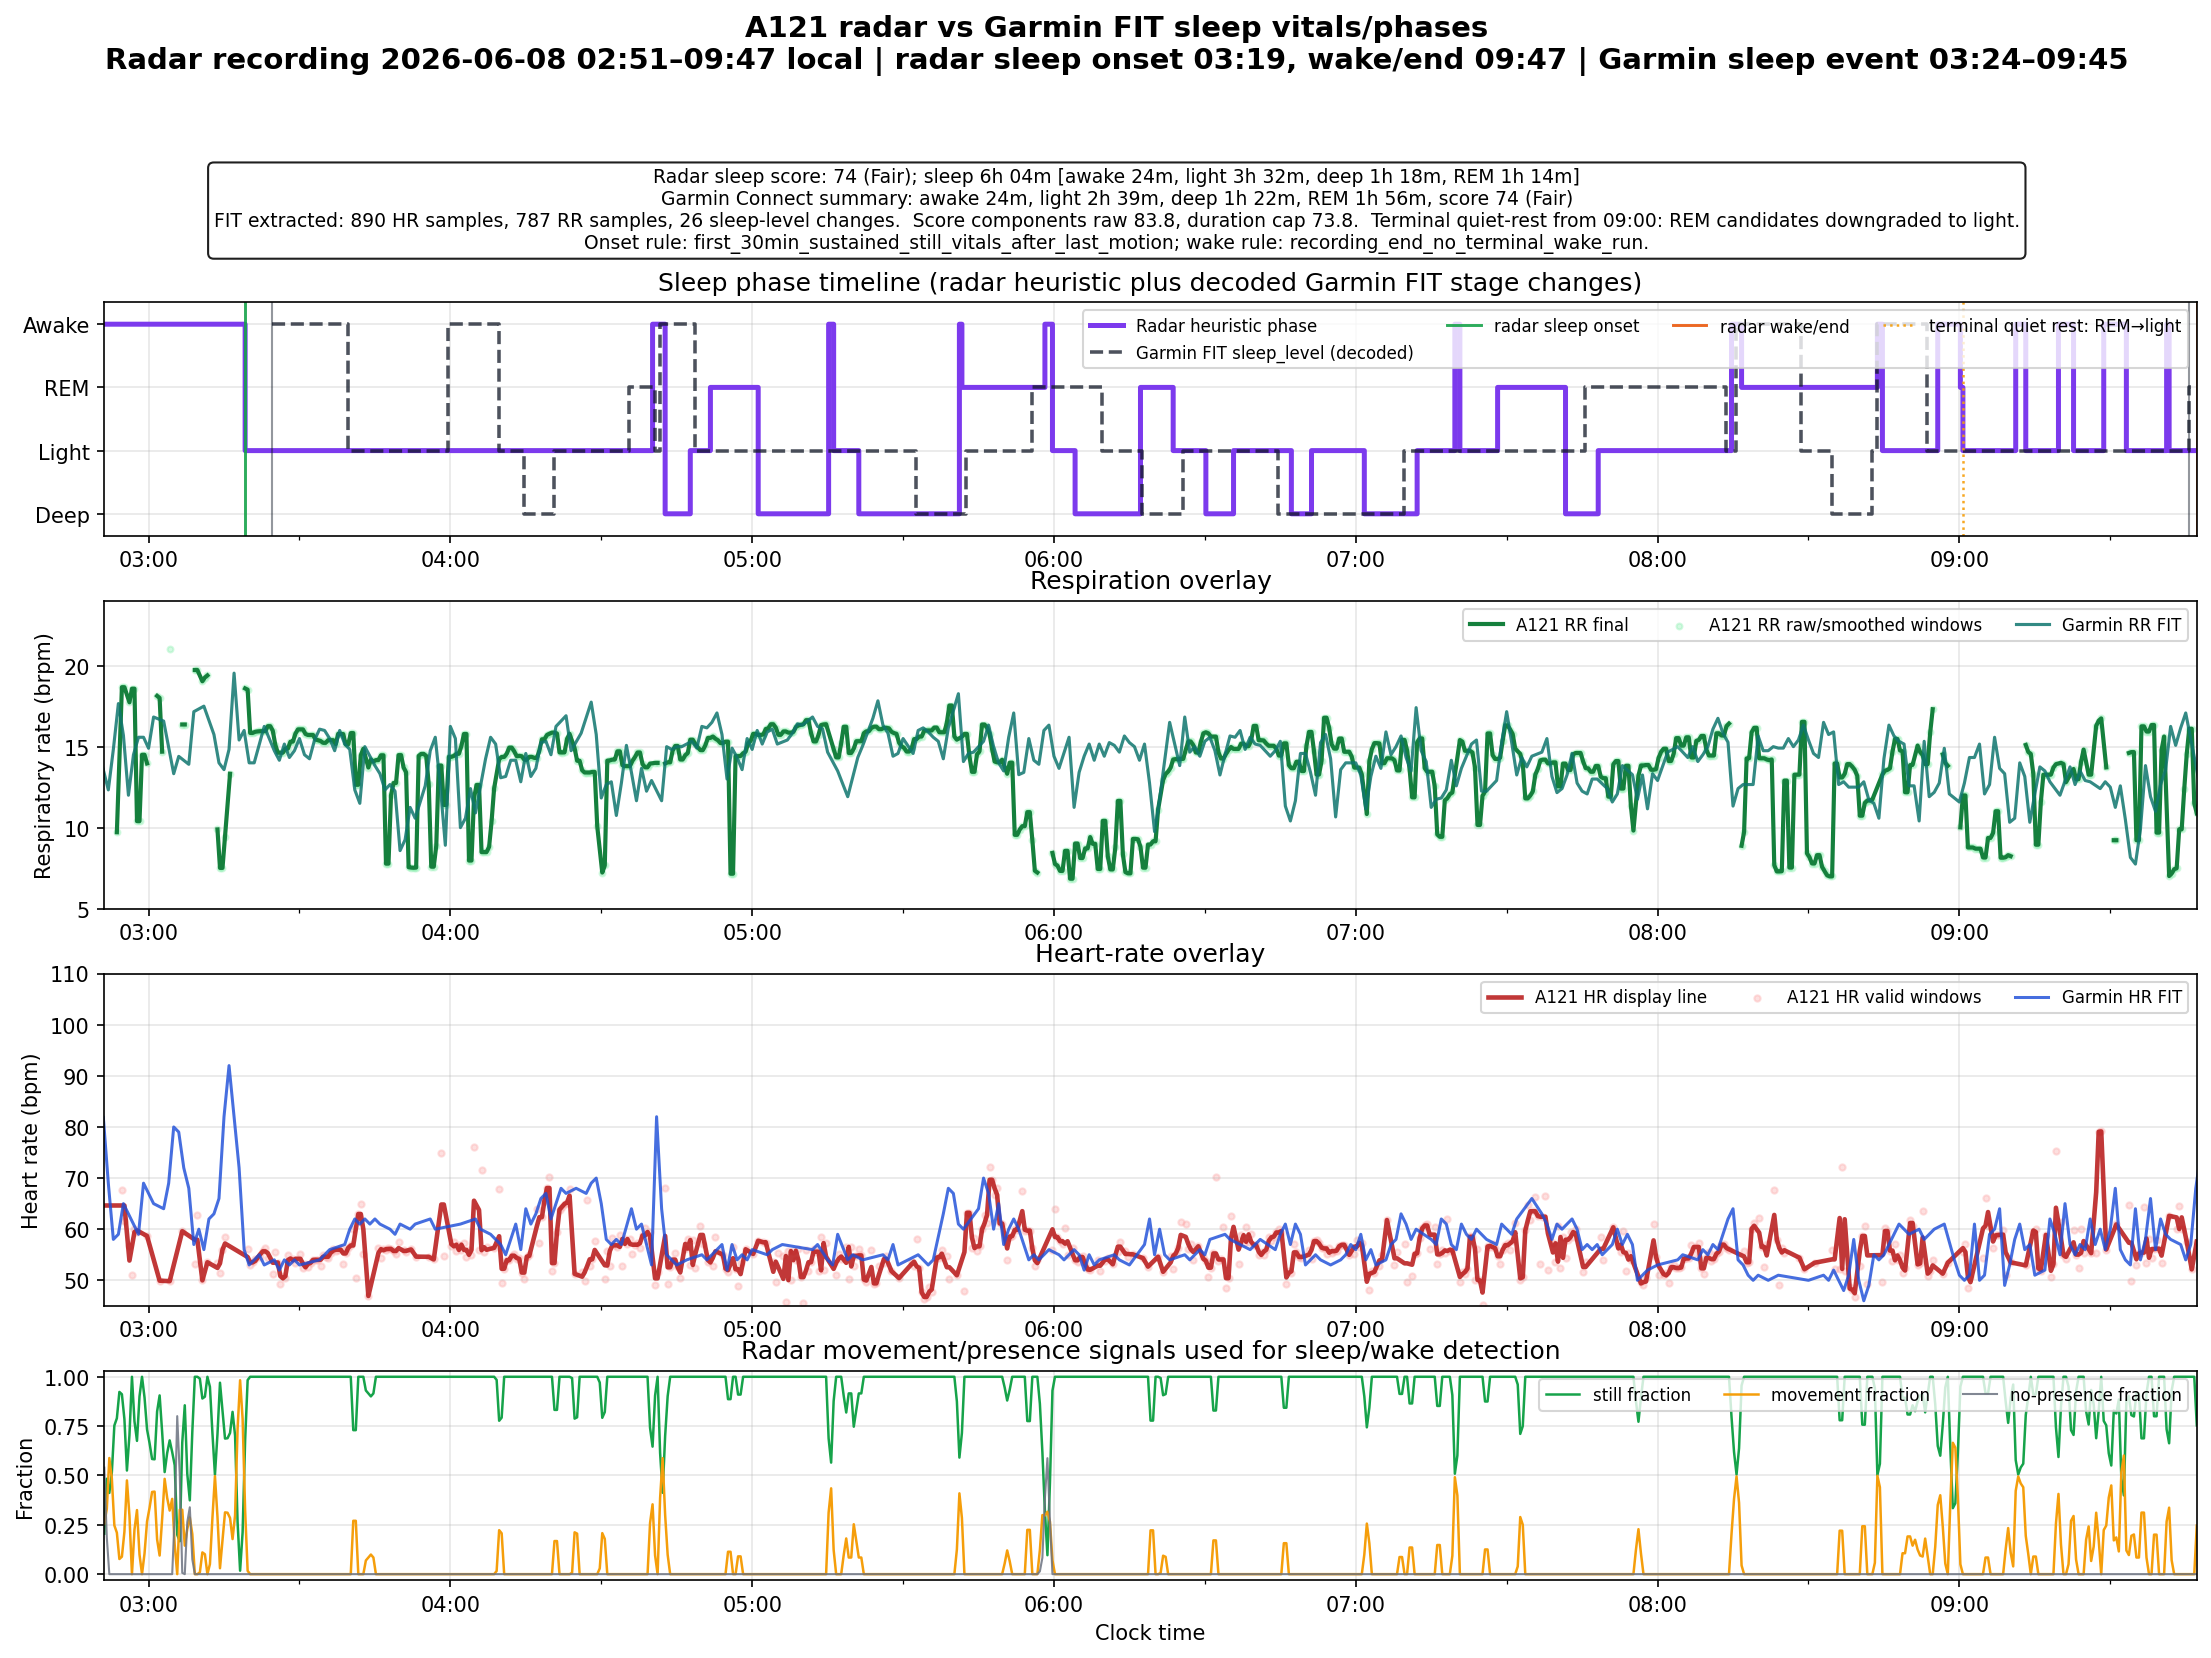
\includegraphics[width=\textwidth]{a121_sleep_sleep-night-1_1-real_2026-06-08_02-50-10_garmin_overlay_sleep_phases.png}
    \caption{Night 1\_1: plano-convex lens. Radar HR/RR and heuristic sleep phases overlaid with Garmin reference data.}
\end{figure}

\begin{figure}[p]
    \centering
    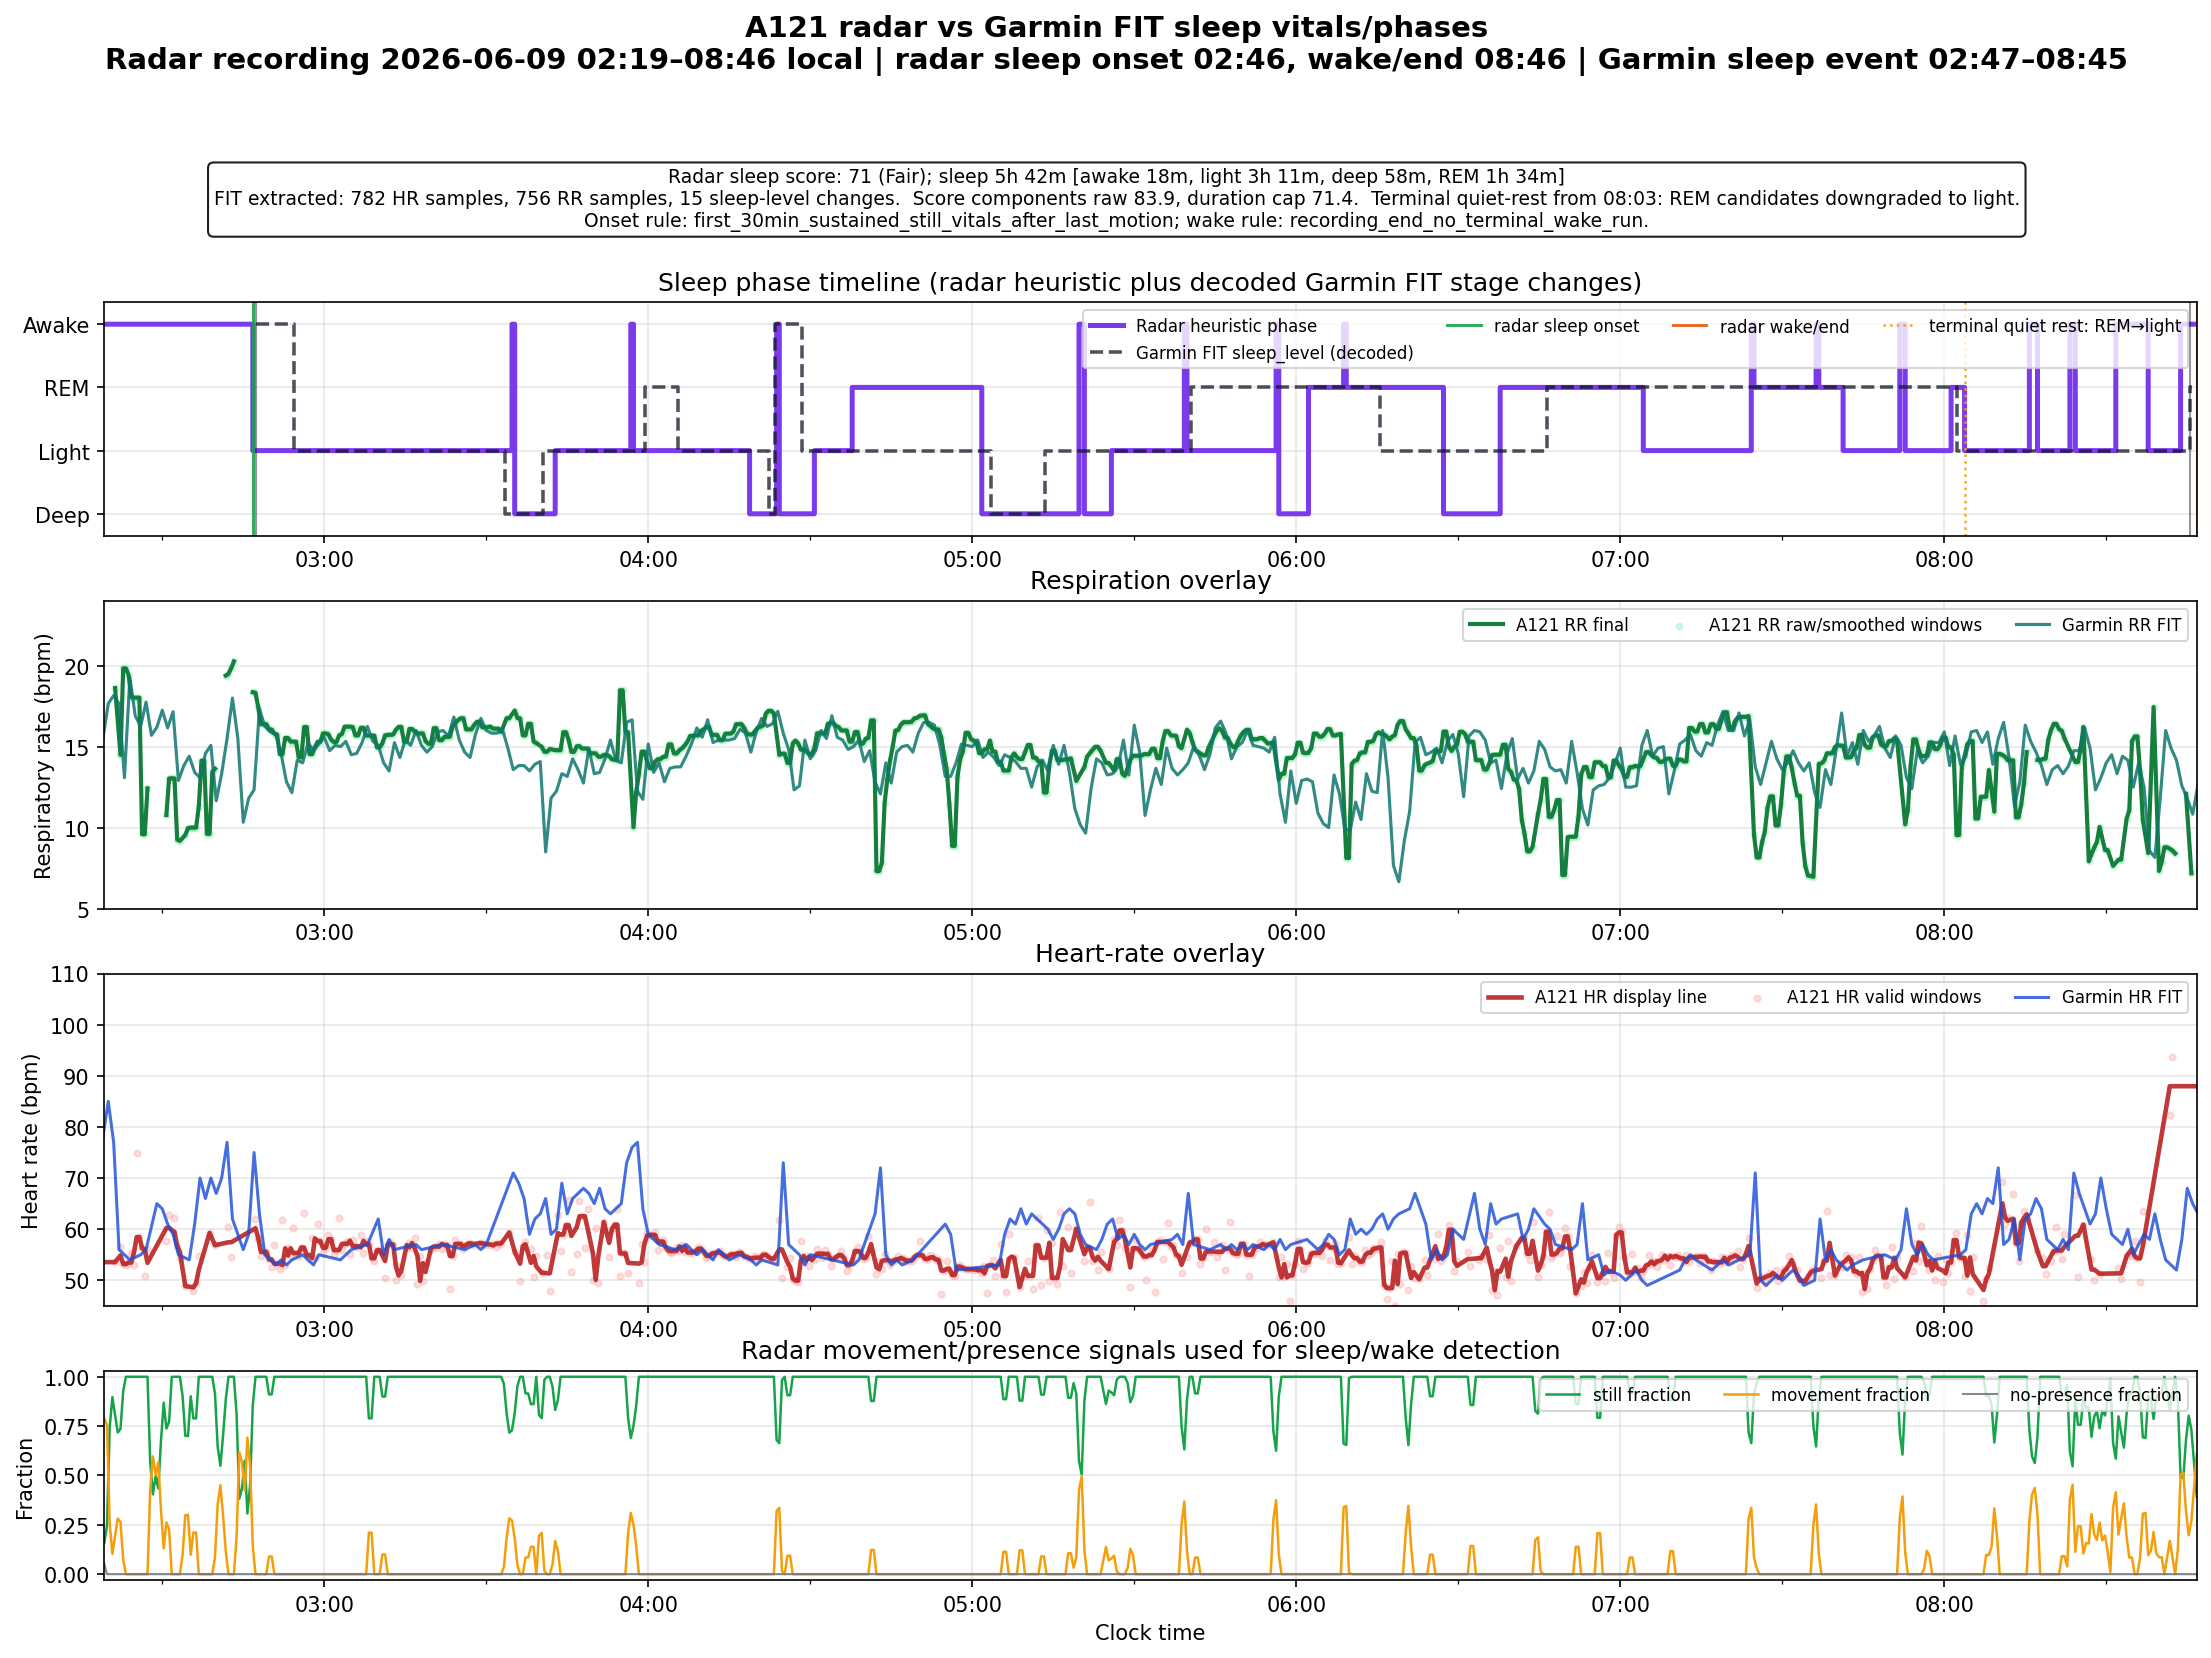
\includegraphics[width=\textwidth]{a121_sleep_sleep-night-2-real_2026-06-09_02-18-14_garmin_overlay_sleep_phases.png}
    \caption{Night 2: FZP lens. This night had high dominant-return amplitude, but the strongest reflector was usually not at the tracked target distance.}
\end{figure}

\begin{figure}[p]
    \centering
    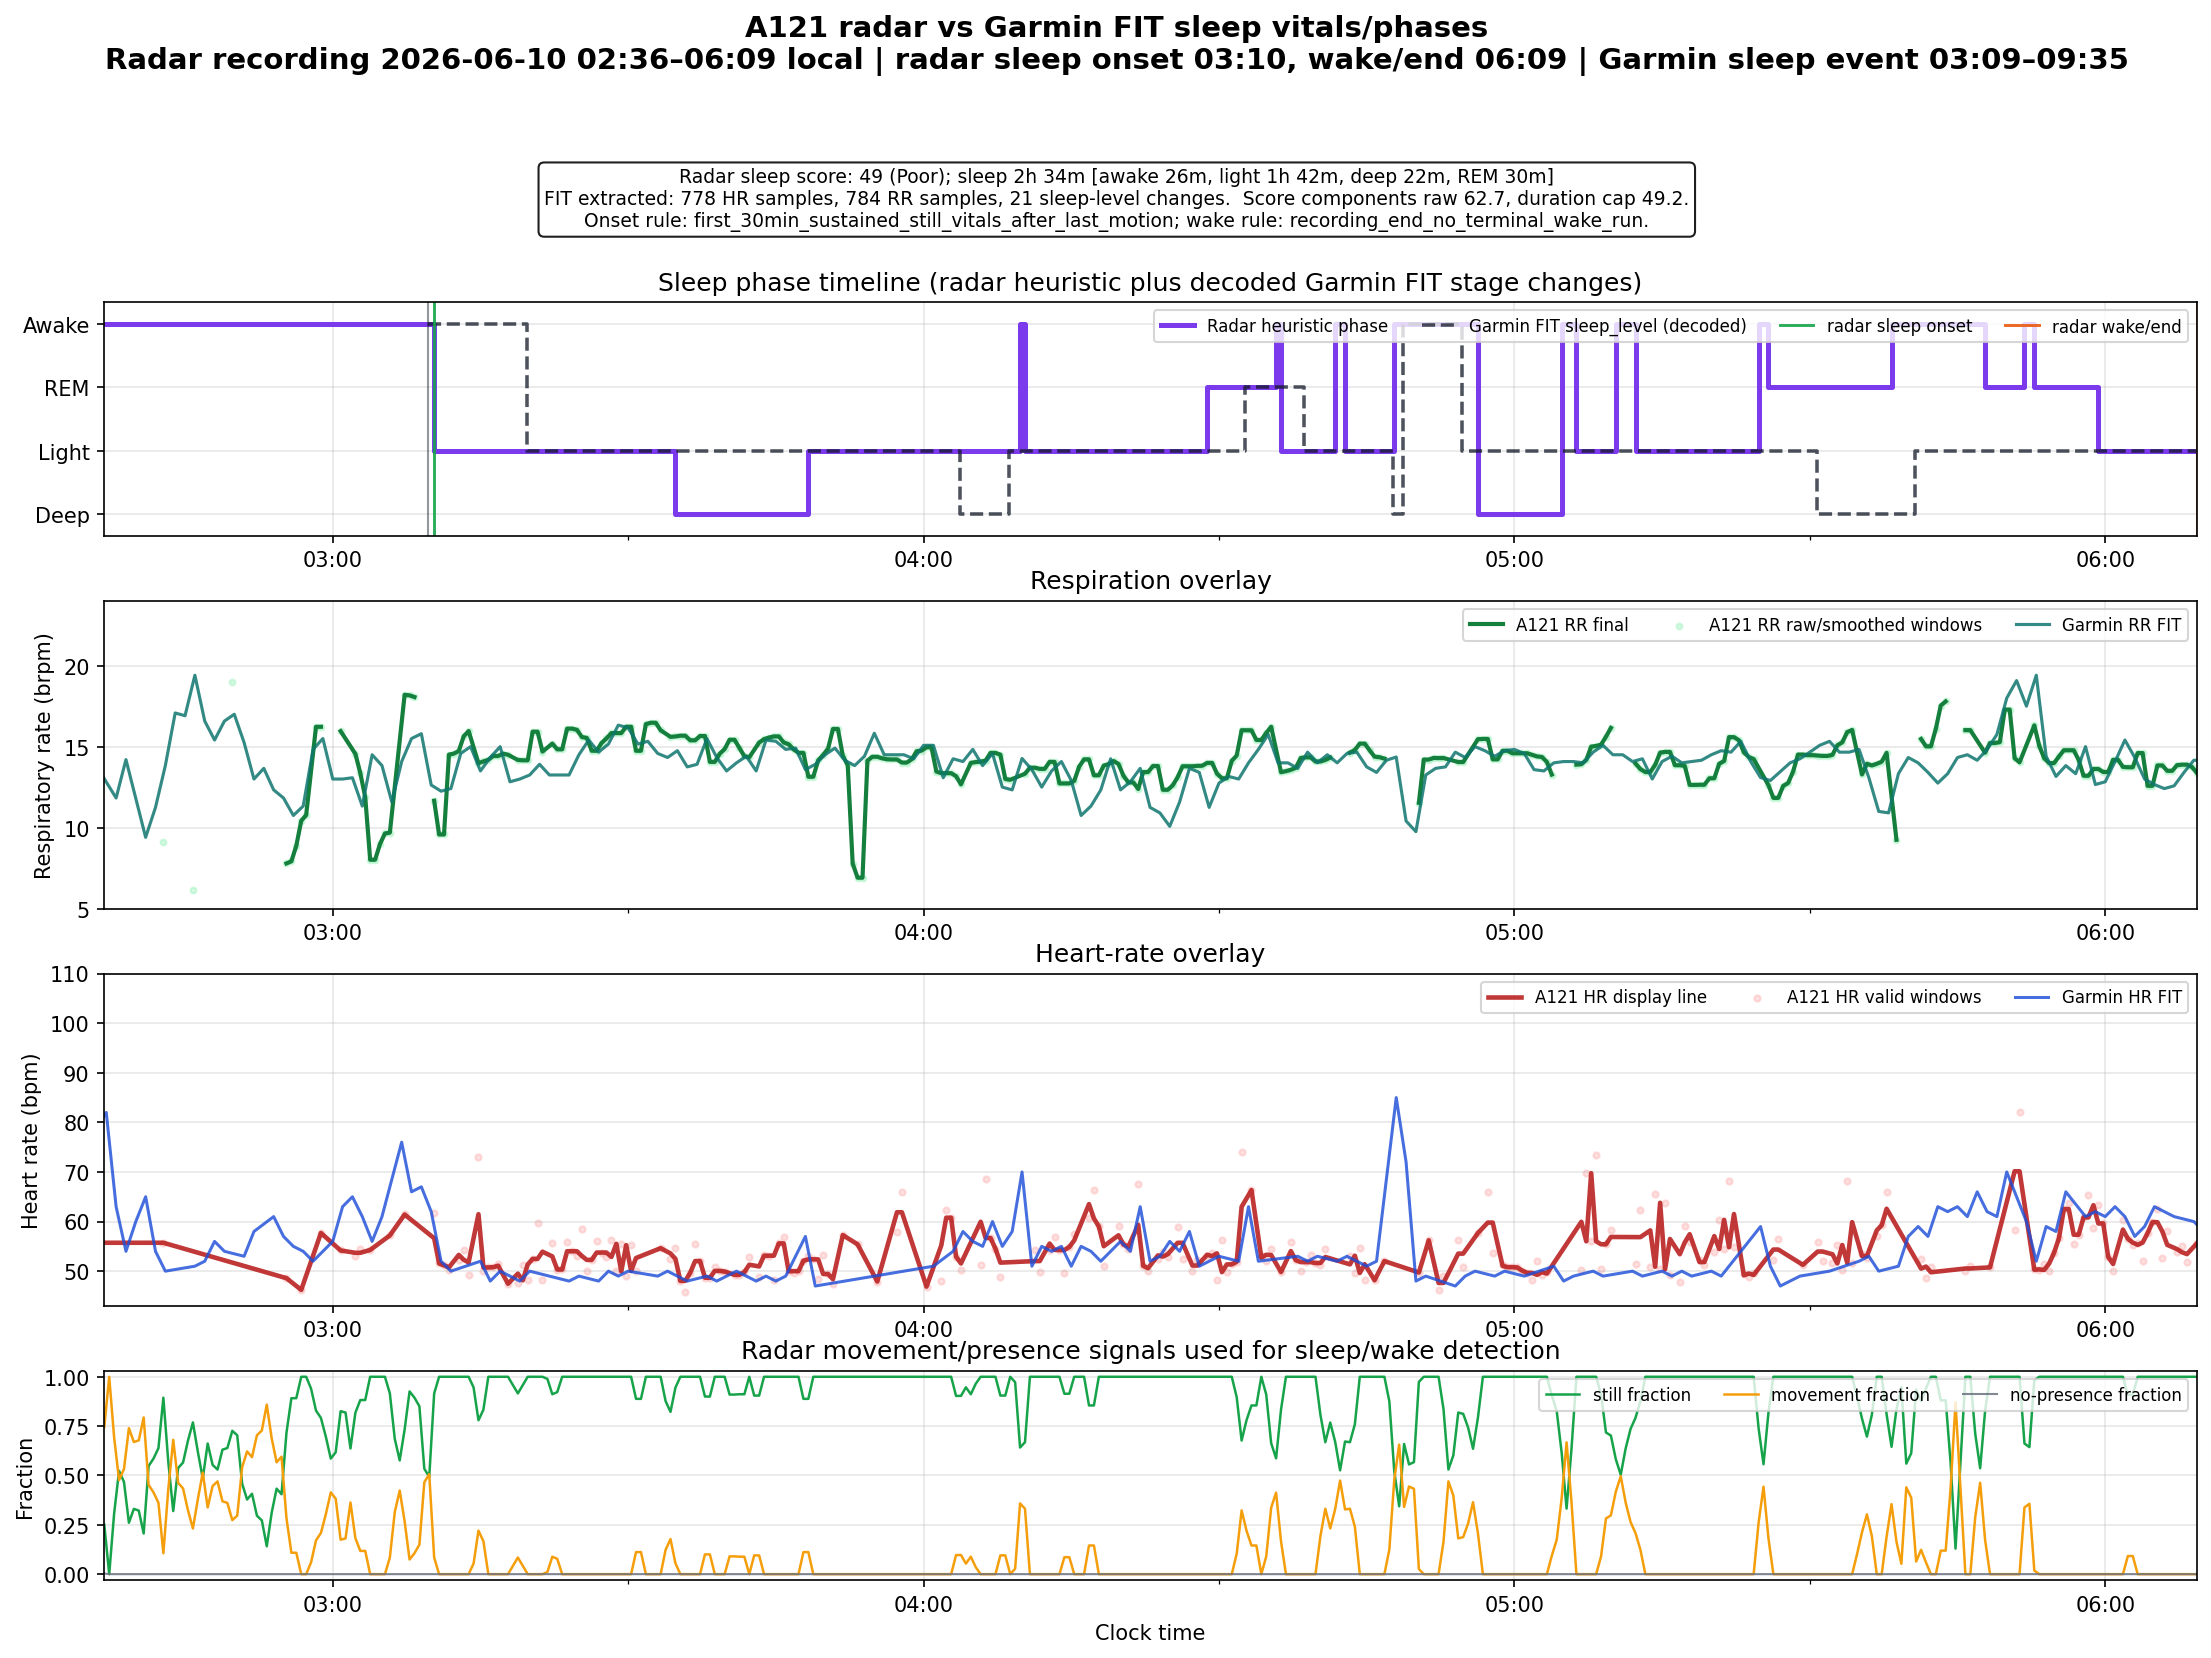
\includegraphics[width=\textwidth]{a121_sleep_sleep-night-3-real-flatcover_2026-06-10_02-35-45_garmin_overlay_sleep_phases.png}
    \caption{Night 3: flat cover / effectively no lens. The recording was interrupted, but the HR agreement with Garmin was the best of the three nights.}
\end{figure}

\begin{figure}[p]
    \centering
    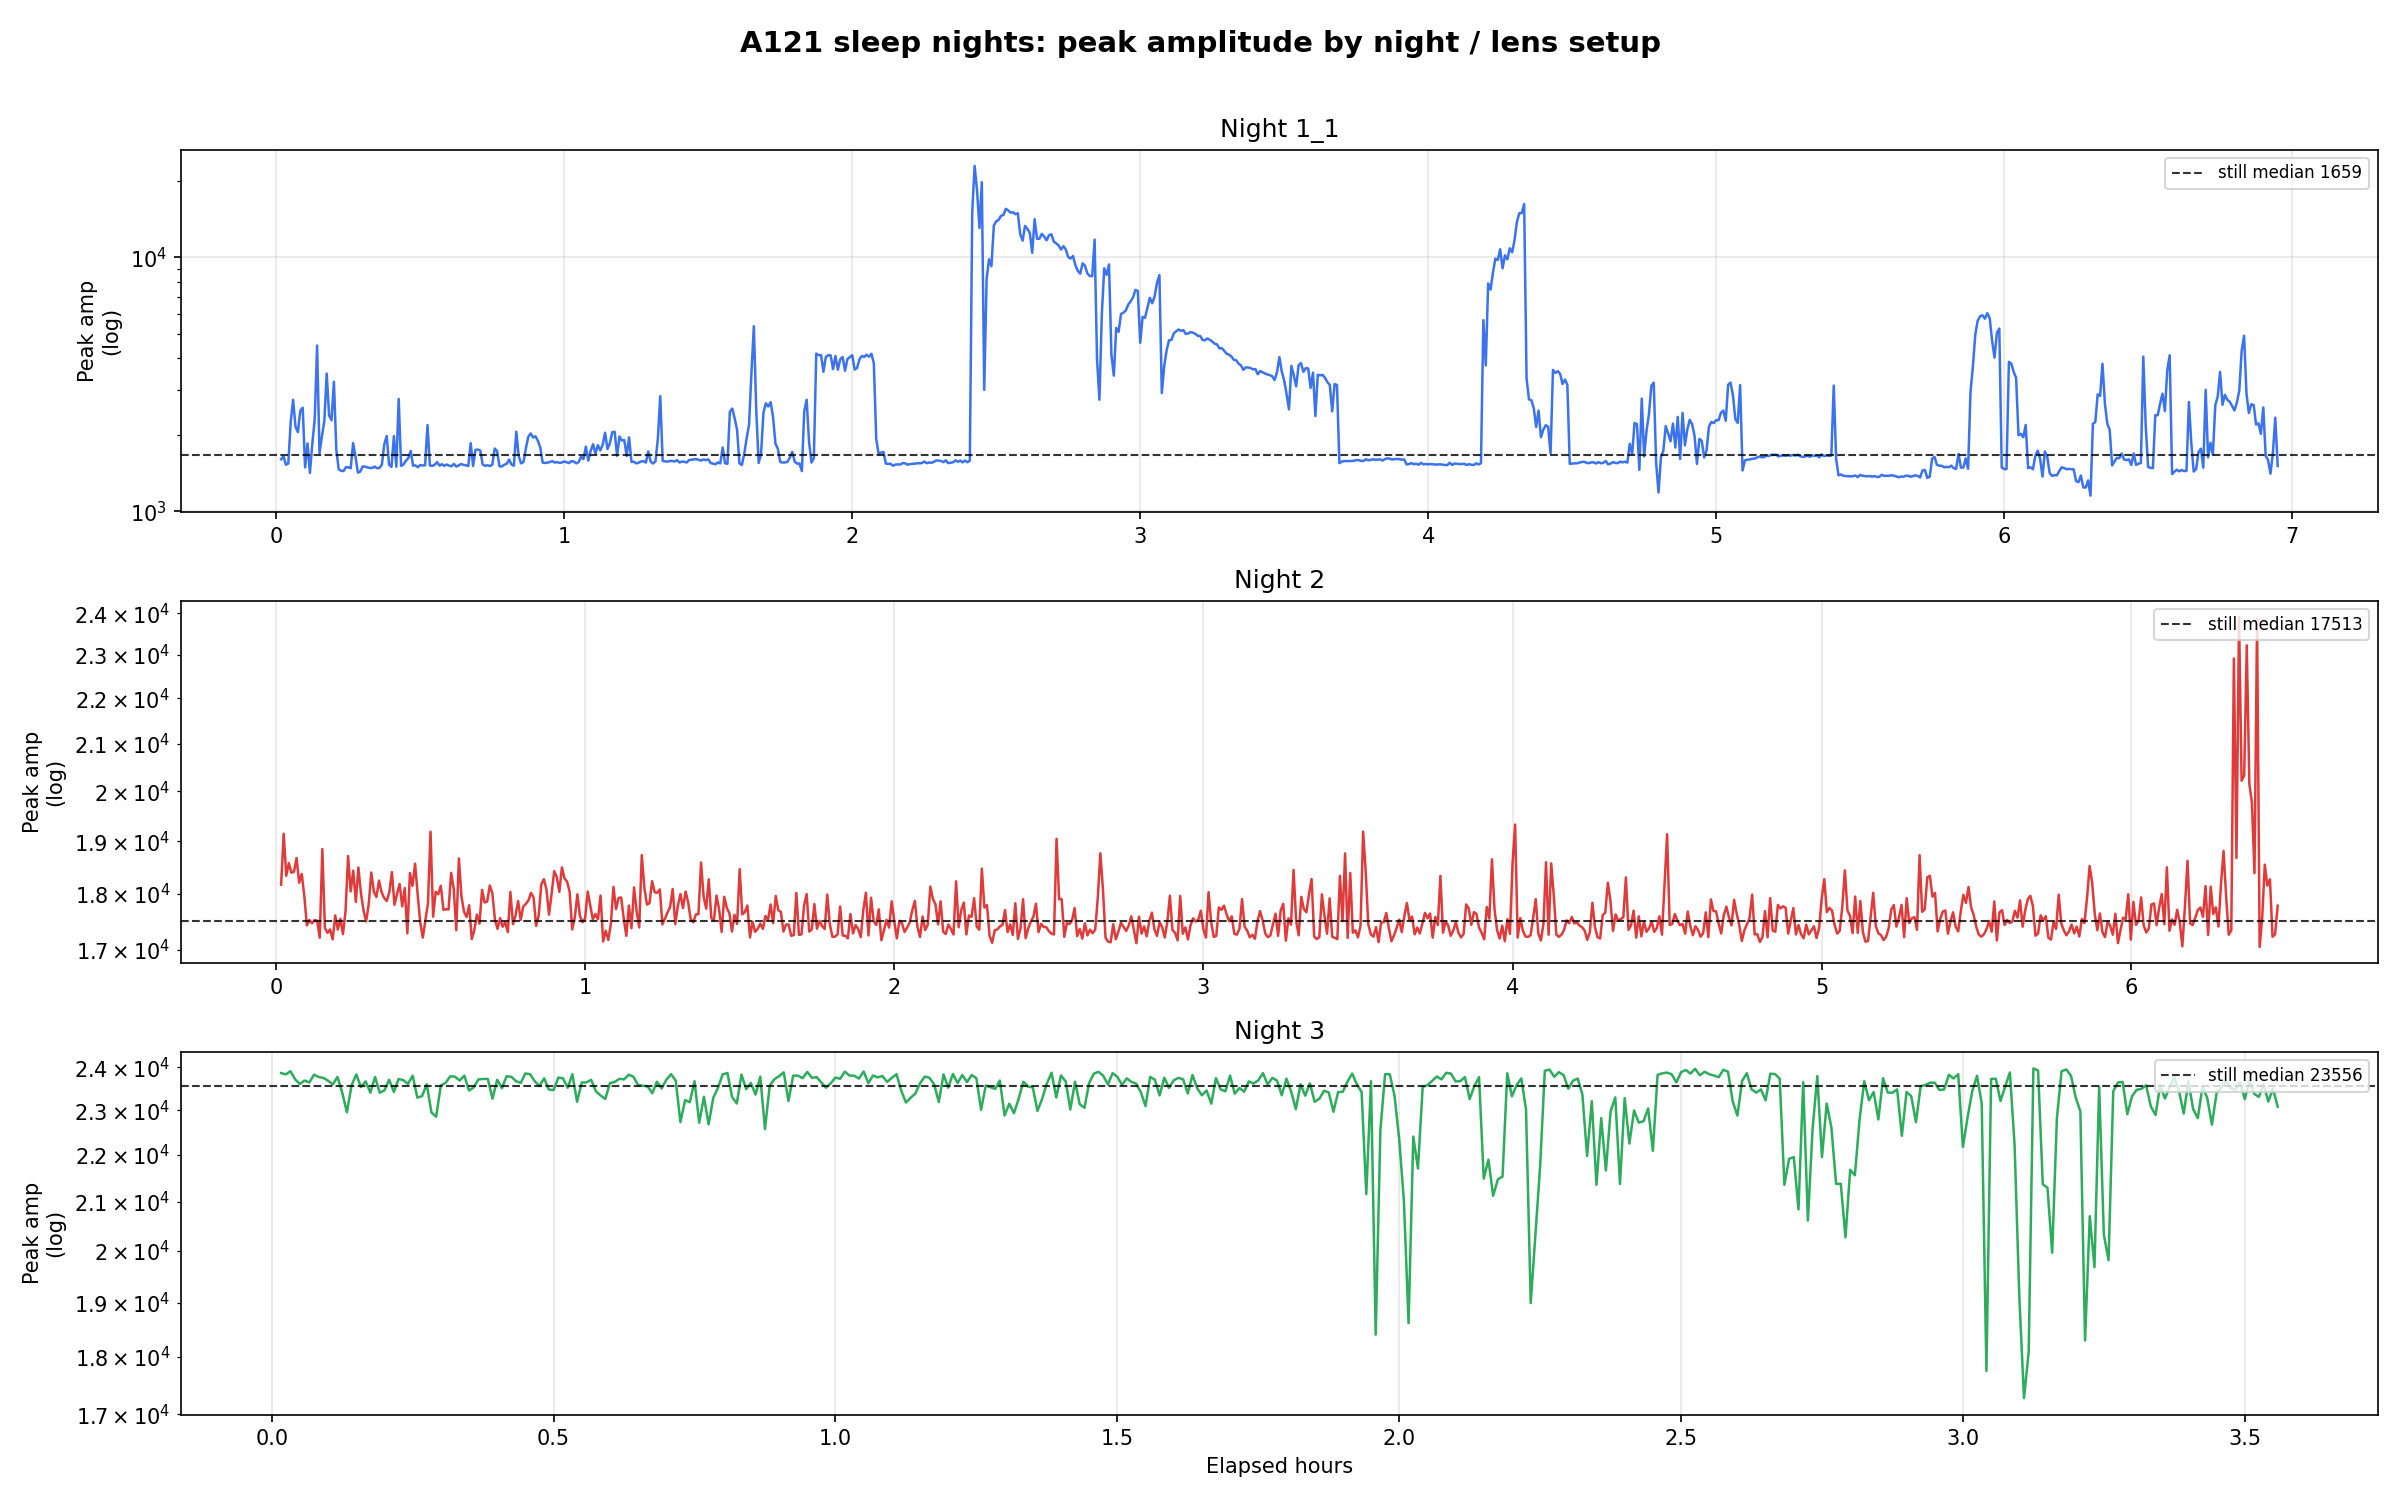
\includegraphics[width=\textwidth]{a121_sleep_peak_amplitude_nights_1_1_2_3.png}
    \caption{Dominant-return peak amplitude across the three overnight recordings. This figure is useful as engineering context, but it should not be read as a direct measure of chest-signal strength.}
\end{figure}

\begin{figure}[p]
    \centering
    \begin{subfigure}[t]{0.49\textwidth}
        \centering
        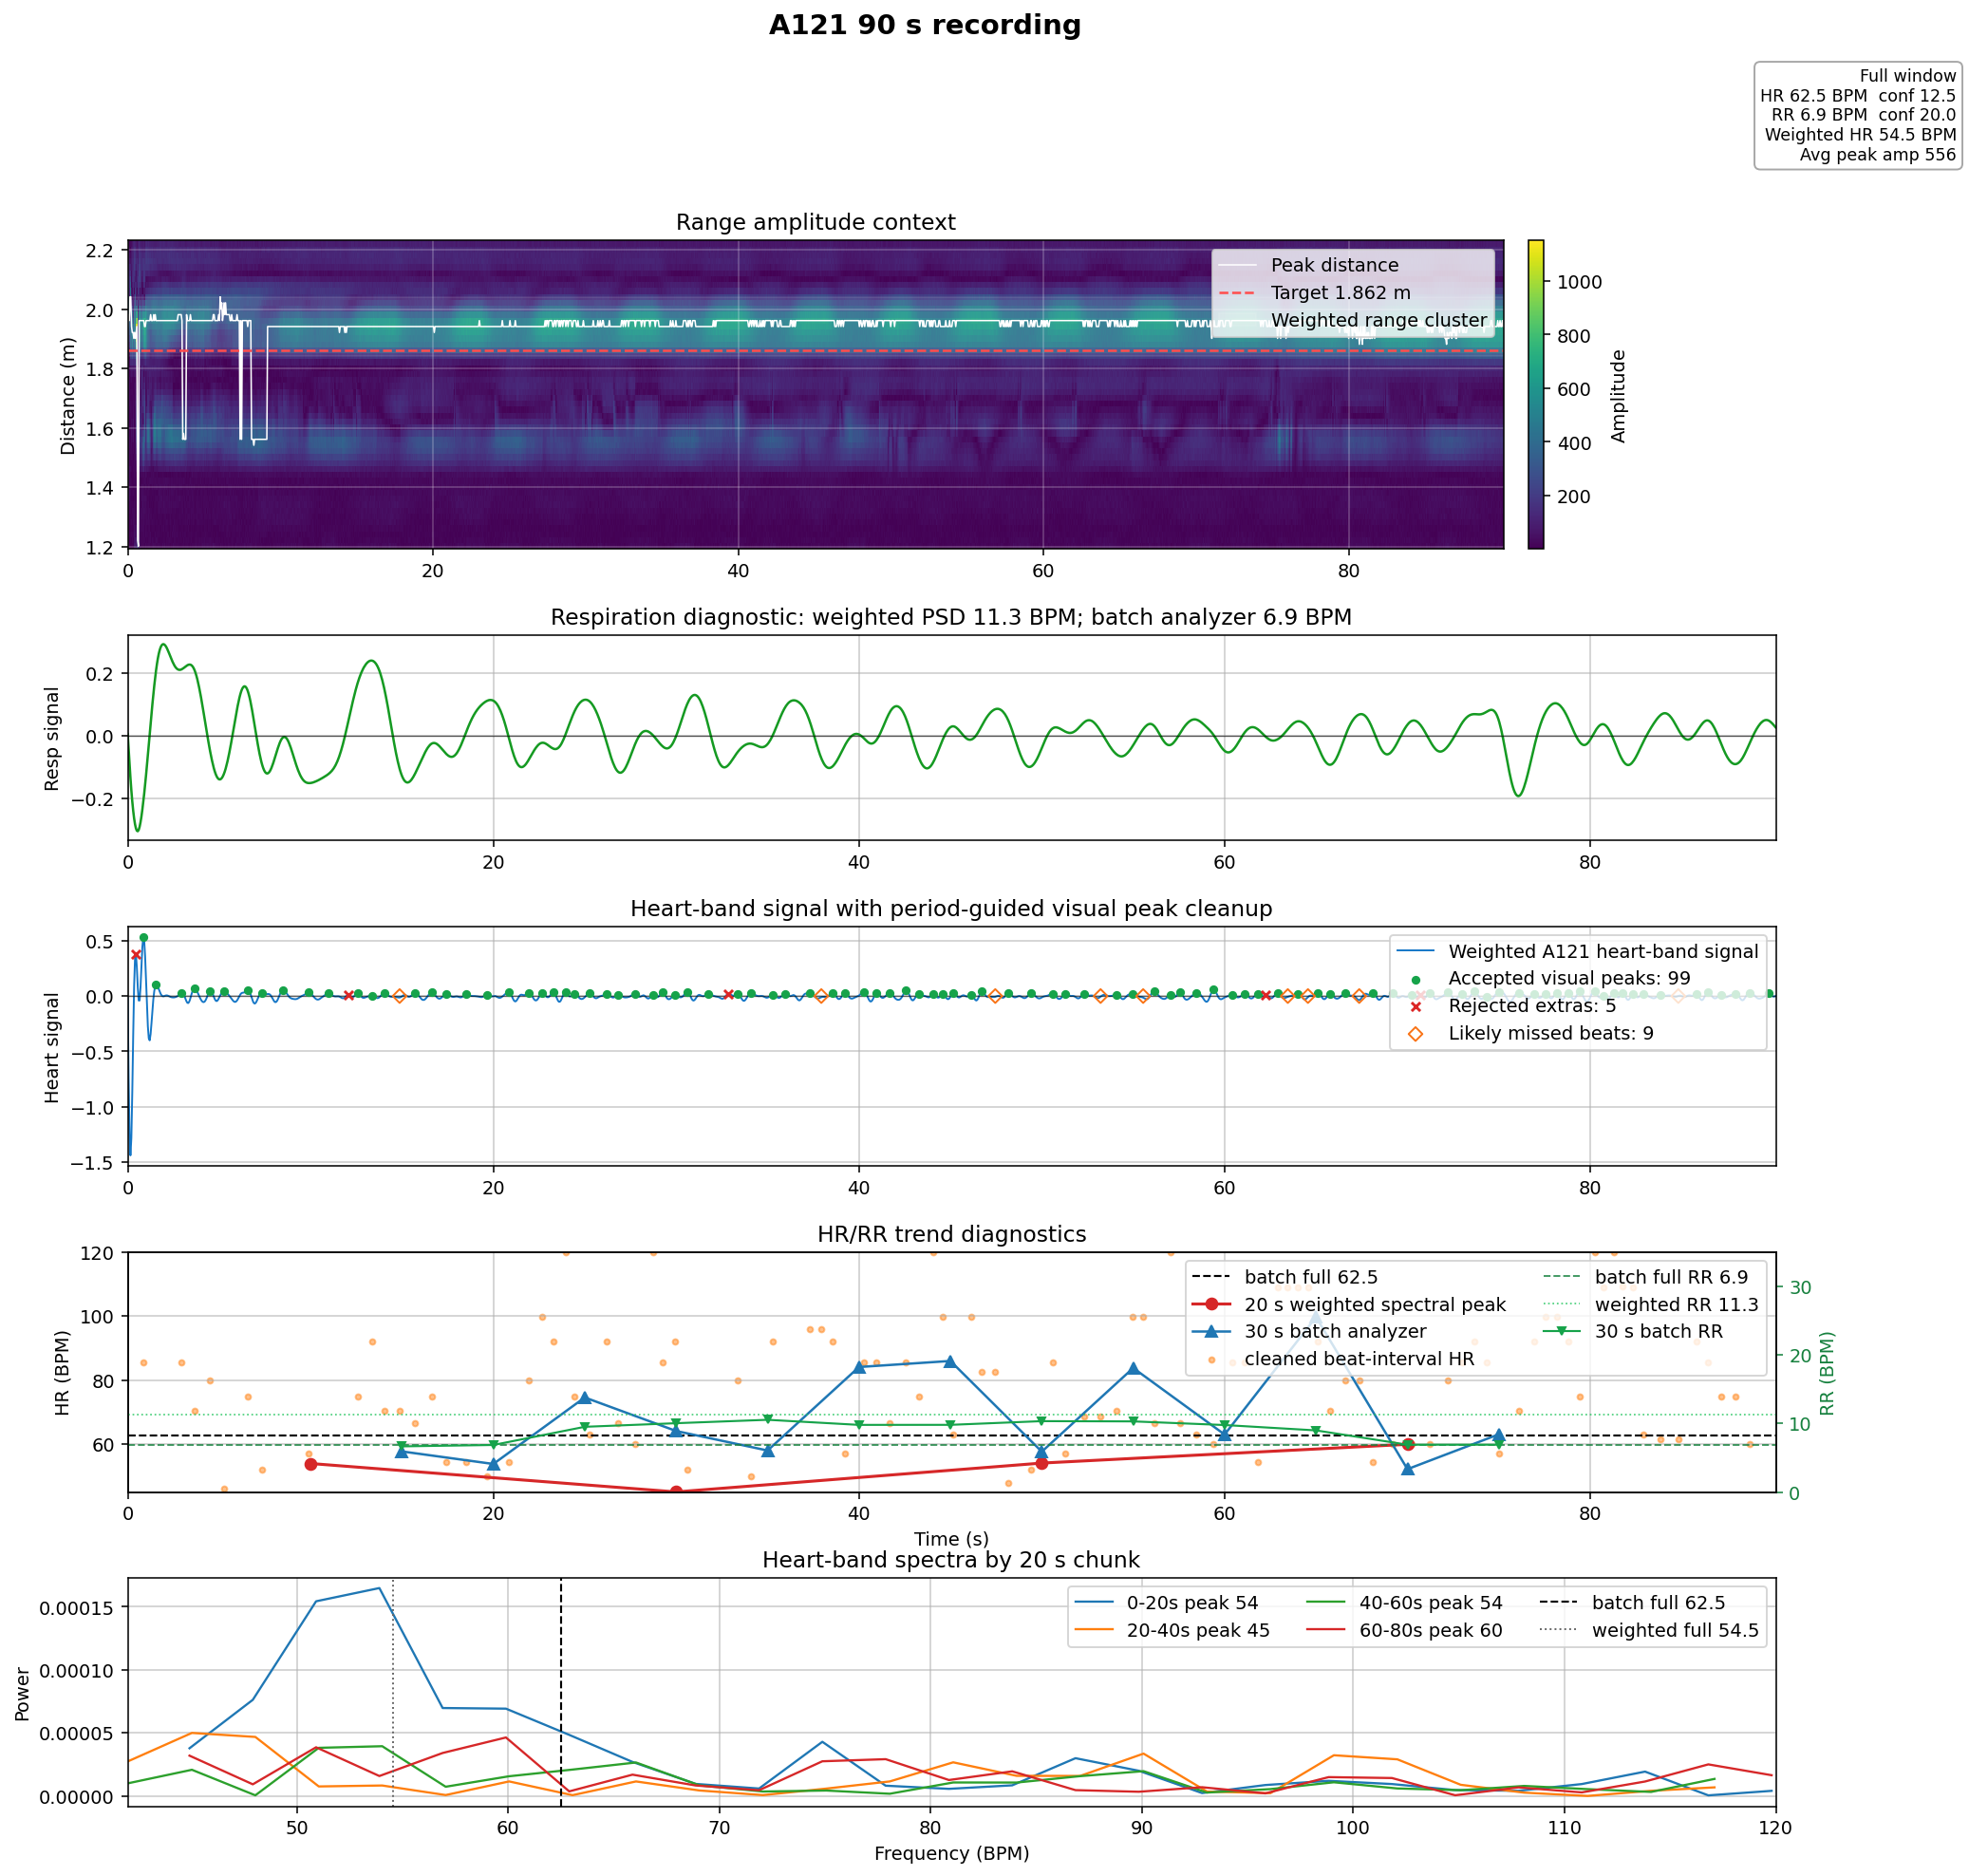
\includegraphics[width=\textwidth]{a121_test_90s_lens-2m-test_2026-06-11_01-44-53_heart_trend.png}
        \caption{Plano-convex lens at about \SI{2}{m}.}
    \end{subfigure}
    \hfill
    \begin{subfigure}[t]{0.49\textwidth}
        \centering
        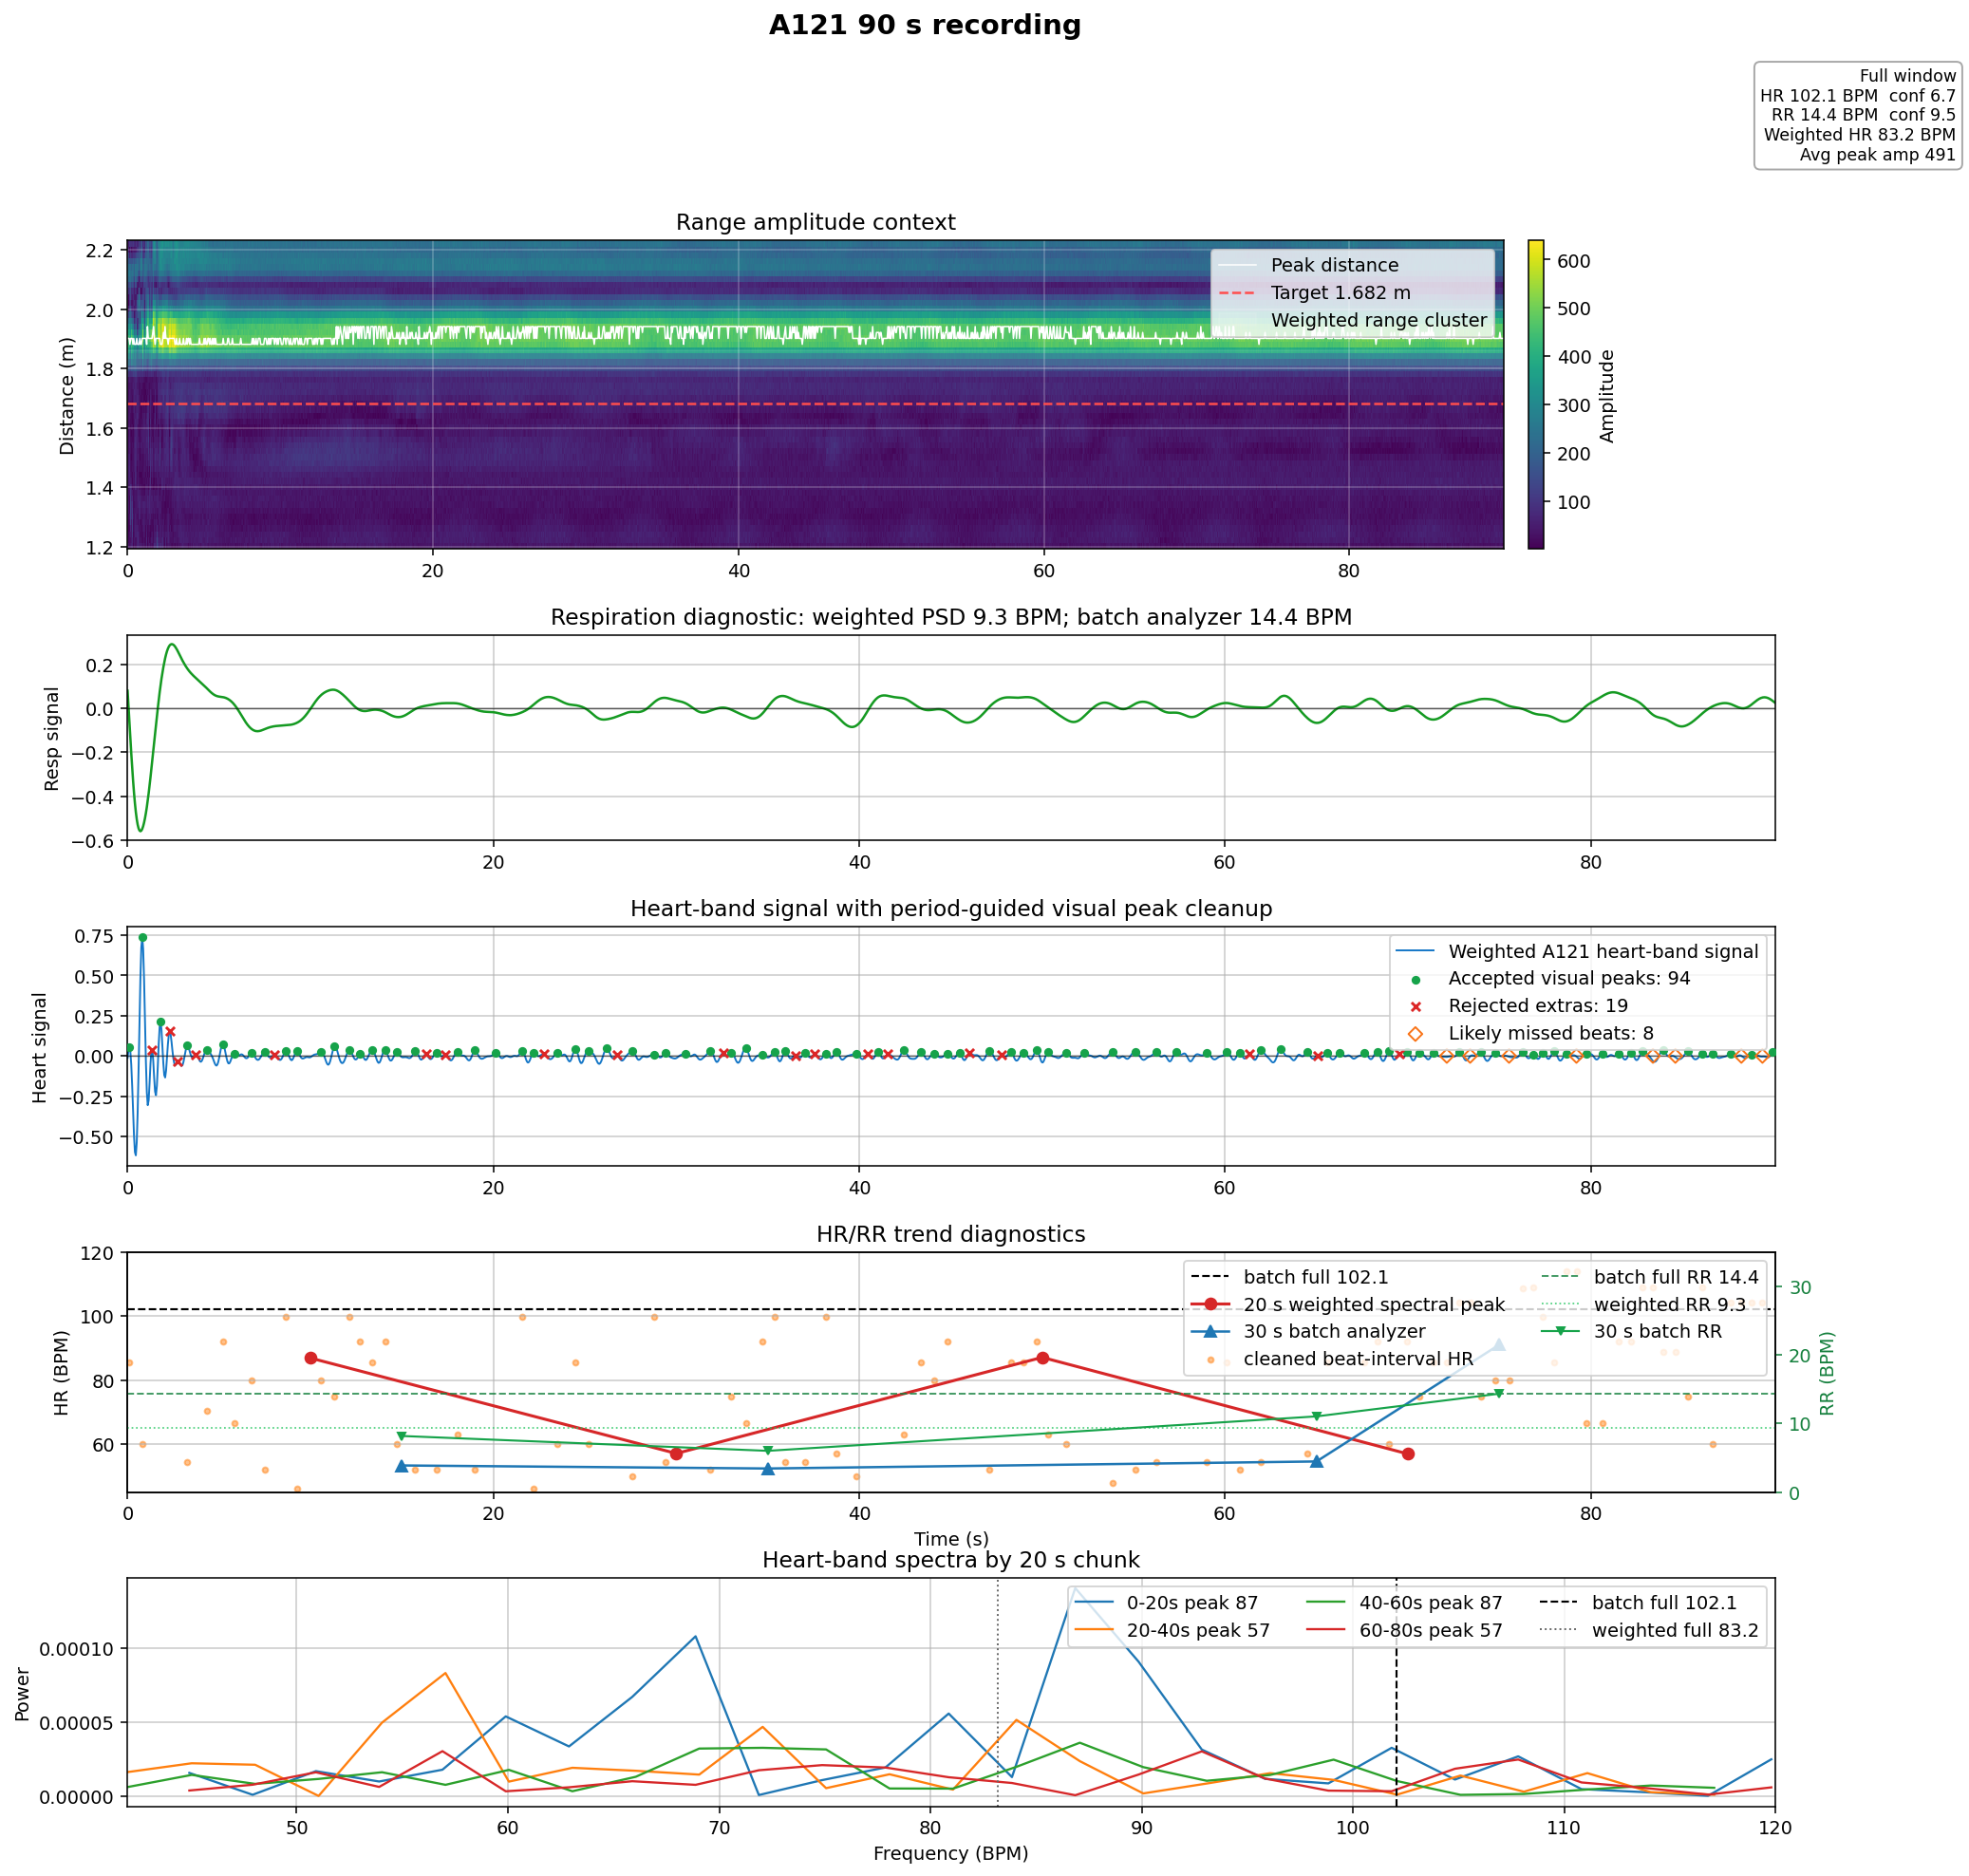
\includegraphics[width=\textwidth]{a121_test_90s_nolens-2m-test_2026-06-11_01-48-43_heart_trend.png}
        \caption{No lens at about \SI{2}{m}.}
    \end{subfigure}
    \caption{Short timed retest used to probe whether the plano-convex lens behaves better when moved farther away to make aiming easier.}
\end{figure}

\section{Discussion}
\subsection{What the Garmin comparison says}
The overnight Garmin comparison is the strongest result available from the current data. RR agreement remained fairly close to Garmin on all three nights, typically within about \SI{0.5}{brpm}. HR was more discriminative: the flat-cover night agreed best with Garmin, while the lensed nights under-read HR by roughly \SIrange{2}{3}{bpm} on average.

\subsection{What the peak amplitudes do \emph{not} say}
The very large raw amplitudes on nights 2 and 3 are not evidence that those nights had stronger physiological returns from the chest. In fact, the target-alignment table suggests the opposite interpretation: the strongest reflector was often spatially separated from the tracked target by \SIrange{0.12}{0.32}{m}. This is fully consistent with a bed-edge setup where the mattress, bed frame, or nearby bedding can dominate the return.

\subsection{What can still be said about the lenses}
The data do not justify a simple ``higher amplitude = better lens'' conclusion. Instead, the results suggest the following:
\begin{itemize}
    \item the plano-convex lens in night 1\_1 may have been mis-aimed and/or used at a geometry that did not place the subject well within the main lobe,
    \item the FZP night produced a very strong dominant reflector but poor target alignment, so the large peak was likely not the subject,
    \item the flat-cover night produced the best HR agreement, which means the simpler configuration was the most reliable in this specific mounting arrangement,
    \item the short \SI{2}{m} retest suggests that moving the lens farther away may improve practical aiming, but the current retest still showed only a small raw amplitude gain.
\end{itemize}

\subsection{REM-to-deep transitions}
The direct REM$\rightarrow$deep transitions seen in the radar heuristic but not in Garmin indicate that the stage classifier should still be treated as exploratory. The HR/RR overlays appear more trustworthy than the exact radar stage labels at this point.

\subsection{Limitations}
This comparison has several limitations:
\begin{itemize}
    \item only one main overnight recording per lens condition,
    \item night 3 was interrupted,
    \item the radar geometry was not fixed in a controlled mechanical jig,
    \item Garmin is a practical consumer reference, not polysomnography,
    \item the dominant-return amplitude was confounded by bed-edge reflections.
\end{itemize}

\section{Overall findings}
The main conclusions of the current experiment are as follows:
\begin{enumerate}
    \item \textbf{Garmin agreement is the correct primary lens-comparison metric for this dataset.} It is substantially more informative than raw dominant-return amplitude.
    \item \textbf{Night 3 (flat cover / effectively no lens) produced the best overnight HR agreement with Garmin.} Nights 1\_1 and 2 under-read HR more clearly.
    \item \textbf{RR tracking was relatively robust across all three nights.} The radar stayed close to Garmin RR regardless of front-end condition.
    \item \textbf{The huge peak amplitudes in nights 2 and 3 were probably dominated by non-subject reflectors.} Target-distance mismatch makes this interpretation much more likely than a true chest-signal gain explanation.
    \item \textbf{The plano-convex lens should be retested with easier aiming geometry.} The later \SI{2}{m} retest supports this plan: the lens did not produce a huge amplitude gain, but it did produce more plausible HR behavior than the no-lens control.
\end{enumerate}

The most useful next step is therefore not to optimize for raw peak amplitude, but to repeat the lens tests with tighter mechanical control, a better defined subject distance, and repeated Garmin-referenced nights per condition.

\begin{thebibliography}{9}
\bibitem{acconeerlens}
Acconeer,
\emph{Lens design}, A121 integration documentation,
\url{https://docs.acconeer.com/en/latest/integration/lens_design.html}.
Key points used here: dielectric lenses shape the beam and increase gain;
plano-convex and FZP example lenses are provided; focal distance may need
tuning because housing/radome effects can shift the gain maximum.
\end{thebibliography}

\end{document}
